\documentclass[../main.tex]{subfiles}
\graphicspath{{\subfix{../}}}
\begin{document}

\chapter{IMF Language: Quick Reference}
\label{ch:IMF visual language}

\begin{figure}
  \centering

  \textbf{Elements}\\[2ex]

  \begin{subfigure}[b]{0.2\textwidth} \centering
    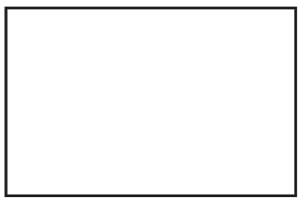
\includegraphics[width=.7\textwidth]{img/IMFmanual-img012.png}
    \caption{Block}
  \end{subfigure}
  \hspace{1cm}
  \begin{subfigure}[b]{0.2\textwidth} \centering
    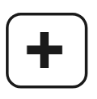
\includegraphics[width=.3\textwidth]{img/IMFmanual-img013.png}
    \caption{Terminal}
  \end{subfigure}
  \hspace{1cm}
  \begin{subfigure}[b]{0.2\textwidth} \centering
    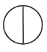
\includegraphics[width=.3\textwidth]{img/IMFmanual-img014.png}
    \caption{Association Point}
  \end{subfigure}

  \par\noindent\rule{.9\textwidth}{0.4pt}\vspace{3ex}

  \textbf{Relations}\\[2ex]
  
  \begin{subfigure}[b]{0.3\textwidth}\centering
    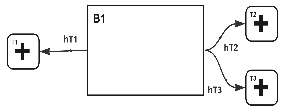
\includegraphics[width=1\textwidth]{img/IMFmanual-img015.jpg}
    \caption{hasTerminal}
  \end{subfigure}
  \hspace{2cm}
  \begin{subfigure}[b]{0.4\textwidth}\centering
    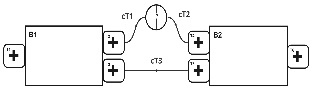
\includegraphics[width=1\textwidth]{img/IMFmanual-img016.jpg}
    \caption{connectedTo}
  \end{subfigure}

  \vspace{1cm}

  \begin{subfigure}[b]{0.3\textwidth}\centering
    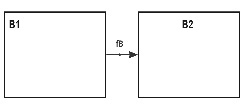
\includegraphics[width=1\textwidth]{img/IMFmanual-img017.jpg}
    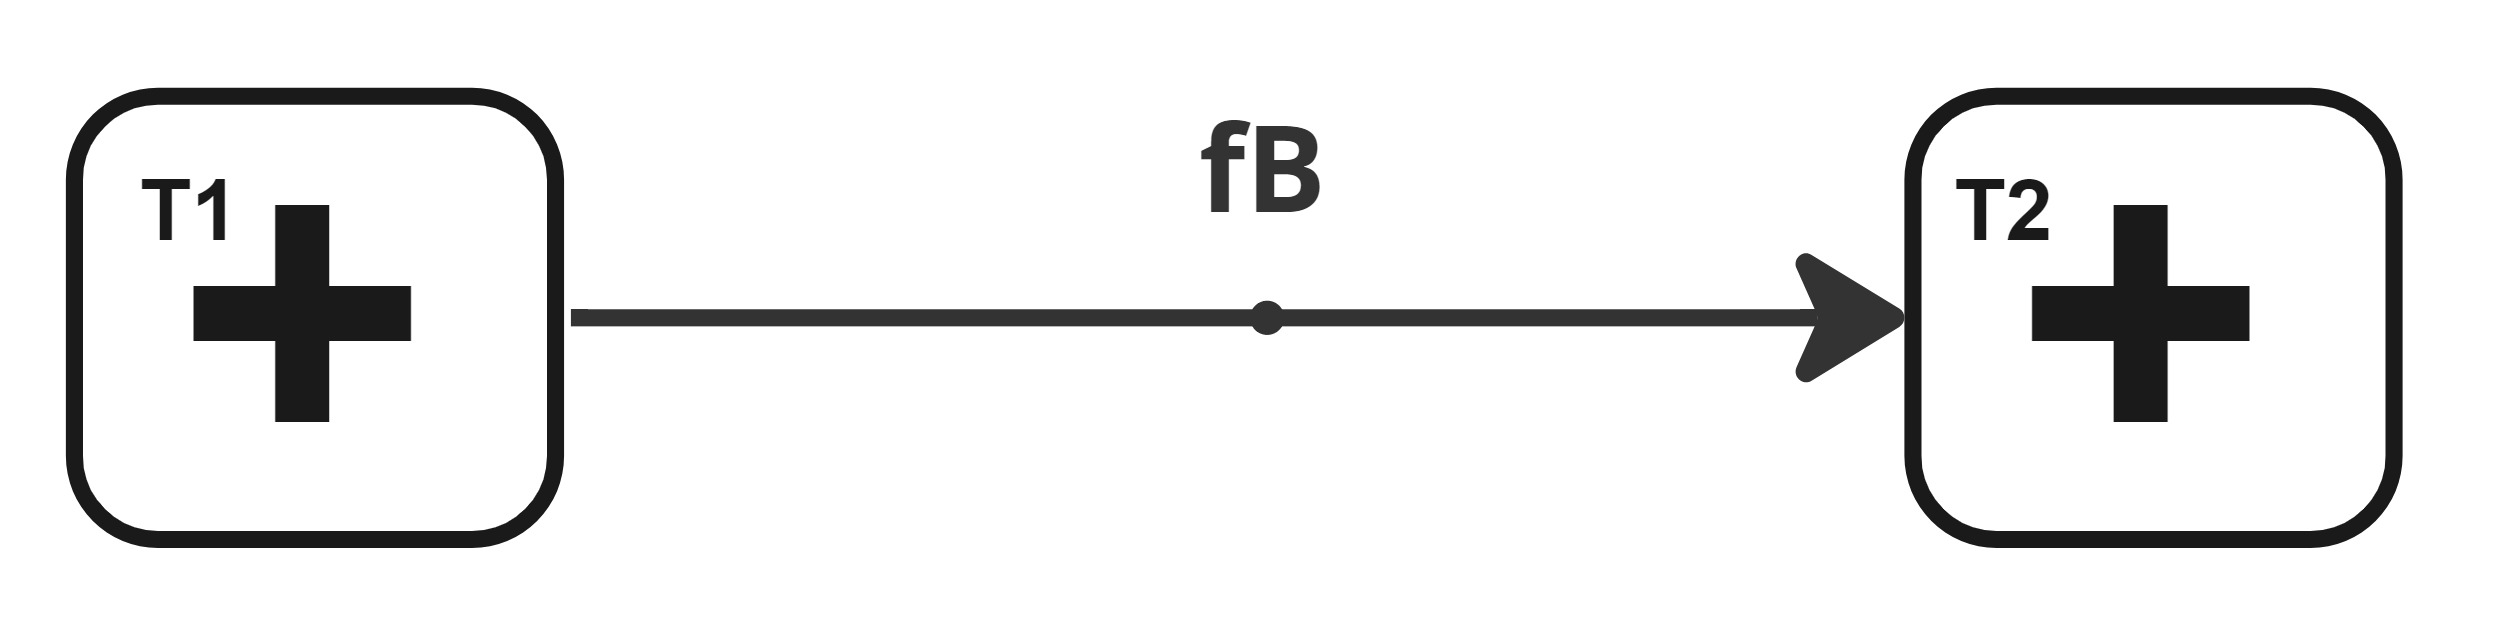
\includegraphics[width=.5\textwidth]{img/IMFmanual-img018.jpg}
    \caption{interAspect}
  \end{subfigure}
  \hspace{2cm}
  \begin{subfigure}[b]{0.3\textwidth}\centering
    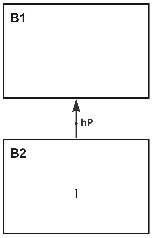
\includegraphics[width=.5\textwidth]{img/IMFmanual-img019.jpg}
    \caption{partOf}
  \end{subfigure}


  \par\noindent\rule{.9\textwidth}{0.4pt}\vspace{3ex}
  
  \textbf{Aspects}\\[2ex]

  \begin{subfigure}[t]{0.2\textwidth}\centering
    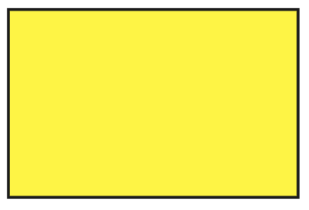
\includegraphics[width=.8\textwidth]{img/IMFmanual-img020.png}
    
\includegraphics[width=.25\textwidth]{img/IMFmanual-img024.png}
    \caption{Function}
  \end{subfigure}
  \hfill
  \begin{subfigure}[t]{0.2\textwidth}\centering
    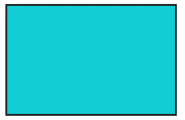
\includegraphics[width=.8\textwidth]{img/IMFmanual-img021.png}
    
\includegraphics[width=.25\textwidth]{img/IMFmanual-img025.png}
    \caption{Product}
  \end{subfigure}
  \hfill
  \begin{subfigure}[t]{0.2\textwidth}\centering
    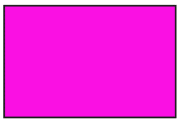
\includegraphics[width=.8\textwidth]{img/IMFmanual-img022.png}
    Terminal is not used\\[1.7ex]
    \caption{Location}
  \end{subfigure}
  \hfill
  \begin{subfigure}[t]{0.2\textwidth}\centering
    
\includegraphics[width=.8\textwidth]{img/IMFmanual-img023.png}
    
\includegraphics[width=.25\textwidth]{img/IMFmanual-img026.png}
    \caption{Installed}
  \end{subfigure}

  \vspace{1cm}
  \caption{An overview of terms and symbols in the IMF language.}
  \label{tab:Table 3}
\end{figure}


\section{Language Elements Overview}

The IMF language consists of 
\begin{itemize}
    \item Aspect elements
    \item Binary relations between aspect elements
\end{itemize}
Aspect elements in an IMF model have been created as instantiations of IMF types and relationships between aspect elements inserted as instances of relations. 

\autoref{tab:Table 3} on page~\pageref{tab:Table 3} gives an overview of terms and symbols in the IMF language.

Note that \autoref{tab:Table 3}  lists  Association Point as an element. This element is not used in the current version of this manual. 

\subsection{Aspect Elements}
An aspect element is either a block or a terminal with exactly one aspect, as
listed in \autoref{tab:Table 6}.

\begin{table}[htb]\centering\caption{The different aspect elements.}\label{tab:Table 6}
  \centering
  \begin{tabularx}{\textwidth}{XXXX}
    \toprule
    &
    {\bfseries Element} &
    {\bfseries Block (B)} &
    {\bfseries Terminal (T)}\\
    \midrule
    {\bfseries Function (F)} &
    Function Element &
    Function Block (FB) &
    Function Terminal (FT)\\
    {\bfseries Product (P)} &
    Product Element &
    Product Block (PB) &
    Product Terminal (PT)\\
    {\bfseries Location (L)} &
    Location Element  &
    Location Block (LB) &
    Location Terminal (LT)\\
    {\bfseries Installed (I)} &
    Installed Element &
    Installed Block (IB) &
    Installed Terminal (IT)\\
    \bottomrule
  \end{tabularx}
\end{table}

%The intended intuition and visualisation for every AspectElements is summarized in \autoref{tab:Table 8} and \autoref{tab:terminals}.

\subsection{Relations  }
Relations in IMF are binary: they connect two aspect elements.
\autoref{tab:Table 4} and
\autoref{tab:Table 7} list all relations with their domain, range and cardinality. 

\begin{table}[htb]
  \centering
  \caption{Summary of partOf and connectedTo relations.}\label{tab:Table 4}
  \begin{tabularx}{\textwidth}{XXXX}
    \toprule
  %  \hline
    {\bfseries Relation} &
    {\bfseries Domain} &
    {\bfseries Range} &
    {\bfseries Cardinality}\\
    \midrule
    {partOf} &
    {Block/Terminal} &
    {Block/Terminal} &
    {Many -- 1}\\
    {connectedTo} &
    {Terminal} &
    {Terminal} &
    {1 -- 1}\\
  \bottomrule\end{tabularx}
\end{table}


\begin{table}[htb]\centering\caption{Inter-aspect relations and their domain and range and
    cardinality.}\label{tab:Table 7}
  %\begin{supertabular}{|m{1.5906599in}|m{1.7621598in}|m{2.0607598in}|m{0.7642598in}|}
  \begin{tabularx}{\textwidth}{XXXX}
        \toprule
    {\bfseries Relation} &
    {\bfseries Domain} &
    {\bfseries Range} &
    {\bfseries Cardinality}\\\midrule
    {{asProduct}} &
    {FunctionElement} &
    {ProductElement} &
    {1 -- many}\\
    {asProduct} &
    {InstalledElement} &
    {ProductElement} &
    {1 -- 1}\\
    {{asFunction}} &
    {ProductElement} &
    {FunctionElement} &
    {1 -- many}\\
    {asLocation} &
    {ProductElement} &
    {LocationElement} &
    {1 -- 1}\\
    {asInstalled} &
    {ProductElement} &
    {InstalledElement} &
    {1 -- many}\\
  \bottomrule\end{tabularx}
\end{table}

\subsection{Visualisation}

A block is visualised as a box, possibly with a collection of attributes written inside. A terminal is visualised as a small box with a plus (+) sign, as shown in \autoref{fig:Figure 16}.

\begin{figure}[htb]
  \centering
  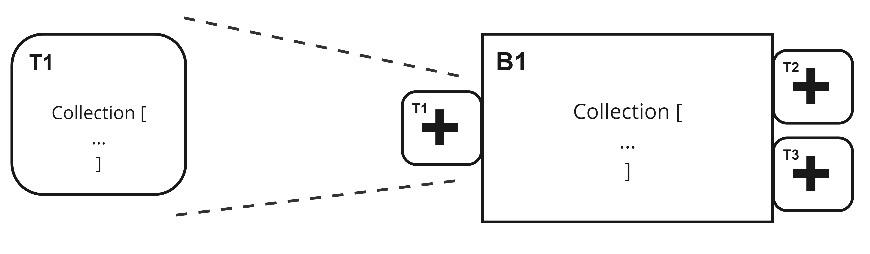
\includegraphics[width=3.94162in,height=1.15217in]{img/ontology/element-terminal.jpg}
  \caption{A terminal.}
  \label{fig:Figure 16}
\end{figure}


A partOf relationship partOf(B2, B1) is illustrated with an arrow pointing from the top of B2 to the bottom of B1, see \autoref{fig:Figure 18}.

\begin{figure}[htb]
  \centering
  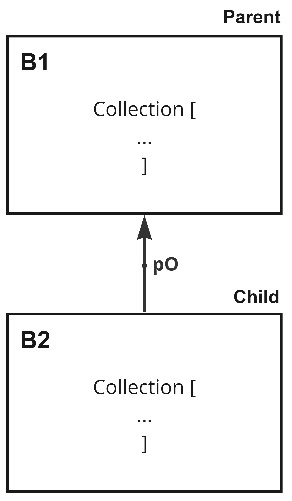
\includegraphics[width=1.3221in,height=2.26735in]{img/ontology/element-partOf.jpg}
  \caption{A partOf relationship between blocks.}
  \label{fig:Figure 18}
\end{figure}

 In this manual a connectedTo relationship is visualised as line between the terminals it connects, as illustrated in
\autoref{fig:Figure 19}.  \autoref{fig:Figure 19} also illustrates 
a connectedTo relationship with
an associated \emph{association point} as a split circle placed in the
middle of the line between the connected terminals. This is not further used in the current version of this manual. 

\begin{figure}[htb]
  \centering
  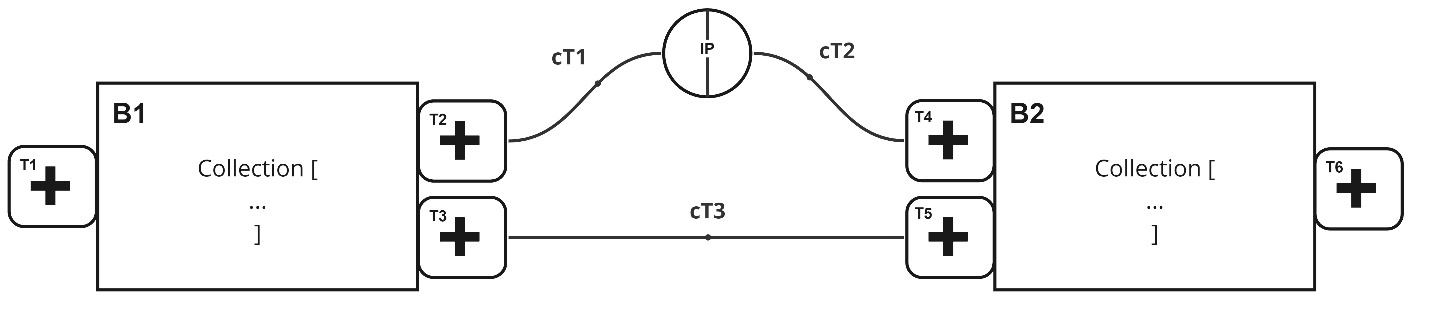
\includegraphics[width=.8\textwidth]{img/ontology/element-connectedTo.jpg}
  \caption{Two connectedTo relationships.}
  \label{fig:Figure 19}
\end{figure}


%Also note that IMF terminology on relations differs from standard set theory in the sense that IMF treats a binary relationship as a separate object and not as an ordered pair. This is called reification, which means that a relationship between two objects is in fact an object in itself. This object is of a special category since it can also be viewed as a relationship. In IMF these objects are called Association points. The association point of a partOf relationship is called a Breakdown point. The association point of a connectedTo relationship is called a Connection point.

In an IMF model the connectedTo and partOf relation
are constrained so that they only relate blocks associated with the same aspect.

The details of the blocks and their interrelations is described in \autoref{ch:The IMF Language Formalized}.


\section{Block}
 Block is the basic building block of the IMF language. A block represents something of interest by
setting the boundaries of anything which is convenient to treat as an entity. This could be a whole industry plant, a
pump system, or a small location of interest.

\autoref{tab:Table 8} summarises the informal interpretation of blocks in each of the reserved aspects. 

%In IMF the basic abstraction mechanism is the concept of a block. A block abstracts the system boundary of a system element. 

\def\rowskp{\\[-1.5ex]}

\begin{table}[htb]\centering\caption{Aspect blocks and their intuition.}\label{tab:Table 8}
  %\begin{supertabular}{|m{1.2996598in}|m{3.75666in}|m{1.2121599in}|}
  \begin{tabularx}{\textwidth}{lX} \toprule
    {\bfseries Name} &
    {\bfseries Intuition}
    % &{\bfseries Graphics}
    \\\midrule
    Function Block (\textbf{FB)} &
    A function block holds the requirements to an intended activity. 
    % & 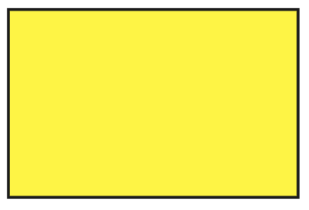
\includegraphics[width=0.7in]{img/IMFmanual-img020.png}
    
    \rowskp
    Product Block (\textbf{PB)} &
    A product block holds the specification of an intended artefact.
    % & 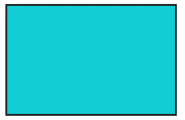
\includegraphics[width=0.7in]{img/IMFmanual-img021.png}

    \rowskp
    Location Block (\textbf{LB)} &
    A location block holds the specification of the spatial extension of an intended artefact. % and requirements imposed by its    spatial position in the Location Breakdown.
    % &  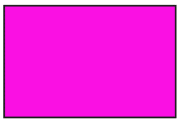
\includegraphics[width=0.7in]{img/IMFmanual-img022.png}
    
    \rowskp
    Installed Block (\textbf{IB)} &
    An installed block holds the documentation of an actually  installed artefact. 
    %&   
\includegraphics[width=0.7in]{img/IMFmanual-img023.png}
    \\
    \bottomrule
  \end{tabularx}
\end{table}

\section{Terminal}
A terminal represents a channel of communication 
%of any type to media, such as information, material, energy) 
for a block; hence a terminal cannot exist without a block. A block may have any number of terminals that each represents a different communication channel or port with which the
block may receive input and/or give output. A terminal that is specified to only receive input is called an
\emph{input terminal}. A terminal that is specified to only give output is called an \emph{output terminal}.
% A
% Terminal that may both
% receive input and give output is called  
% a \textit{bidirectional} Terminal, or, simply, a Terminal.  

\autoref{tab:terminals} summarises the informal interpretation of terminals in each of the reserved aspects. 


\begin{table}[htb]\centering\caption{Aspect terminals and their intuition.}\label{tab:terminals}
  \begin{tabularx}{\textwidth}{lX}
        \toprule
    
    {\bfseries Name} &
    {\bfseries Intuition}
    %&{\bfseries Graphics}
    \\ \midrule
    Function Terminal (\textbf{FT}) &
    Requirements to one input/output stream state of a intended activity
    % & \centering\arraybslash  
\includegraphics[width=0.35063in,height=0.33245in]{img/IMFmanual-img024.png}
    
    \rowskp
    Product Terminal (\textbf{PT}) &
    Specification of one input/output/bidirectional terminal of an intended artefact
    %& \centering\arraybslash  
\includegraphics[width=0.33351in,height=0.33351in]{img/IMFmanual-img025.png}

    \rowskp
    Location Terminal (\textbf{LT}) &
    Not used
    %& \centering\arraybslash Not used

    \rowskp
    Installed Terminal (\textbf{IT}) &
    Documentation of an actually installed artefact terminal.
    % &\centering\arraybslash  
\includegraphics[width=0.34253in,height=0.3131in]{img/IMFmanual-img026.png}
    \\
  \bottomrule\end{tabularx}
\end{table}

\section{hasTerminal}

\autoref{tab:hasTerminal} summarises the informal interpretation of hasTerminal relationships in each of the reserved aspects. 


%\autoref{tab:partOf} to \autoref{tab:connectedTo} give overview of the different relations between Aspect Elements and their intuitions.



\begin{table}[htb]\centering\caption{hasTerminal relations and their intuition.}\label{tab:hasTerminal}
  \begin{tabularx}{\textwidth}{lX}%{|m{1.1975598in}|m{0.90595984in}|m{4.00386in}|}
        \toprule
    
    \textbf{Relationship} &
    {\bfseries Intuition}\\
    \midrule
    hasTerminal(\textbf{FB},\textbf{FT}) &
    The media state of function terminal \textbf{FT} is the input/output of the intended activity in function block \textbf{FB}

\rowskp
    hasTerminal(\textbf{PB},\textbf{PT}) &
    The product terminal \textbf{PT} is a specification of one input/output terminal of the intended artefact of product block
    \textbf{PB}

\rowskp
    hasTerminal(\textbf{LB},\textbf{LT}) &
    Not used

\rowskp
    hasTerminal(\textbf{IB},\textbf{IT}) &
    The actually installed terminal \textbf{IT} holds documentation of an actually installed artefact terminal \textbf{IB}\\
  \bottomrule\end{tabularx}
\end{table}

\section{partOf}


\begin{table}[htb]\centering\caption{partOf relations and their intuition.}\label{tab:partOf}
  \begin{tabularx}{\textwidth}{lX}%{|m{1.1975598in}|m{4.94136in}|}
        \toprule
    
    {\bfseries Relationship} &
    {\bfseries Intuition}\\
    \midrule
    partOf(\textbf{FB1},\textbf{FB2}) &
    The intended activity of function block \textbf{FB1} is a sub-activity of that of function block \textbf{FB2}

\rowskp
    partOf(\textbf{PB1},\textbf{PB2}) &
    The intended artefact of product block \textbf{PB1} is a sub-assembly of the intended artefact of product block \textbf{PB2}

\rowskp
    partOf(\textbf{LB1},\textbf{LB2}) &
    The intended location of location block \textbf{LB1} is located in the intended location of location block \textbf{LB2}

\rowskp
    partOf(\textbf{IB1},\textbf{IB2}) &
    The actually installed artefact of installed block \textbf{IB1} is sub-assembly of the actually installed artefact of installed block \textbf{IB2}\\
  \bottomrule\end{tabularx}
\end{table}
The partOf relation promotes a System-Of-Systems way of thinking, cf. \autoref{sec:Breakdown}. 

\autoref{tab:partOf}
summarises the informal interpretation of partOf relationships in each of the reserved aspects. 

\section{connectedTo}

\autoref{tab:connectedTo}
summarises the informal interpretation of connectedTo relationships in each of the reserved aspects. 




\begin{table}[htb]
\centering
\caption{connectedTo relations and their intuition.}
\label{tab:connectedTo}
  \begin{tabularx}{\textwidth}{lX}%{|m{1.2962599in}|m{1.0038599in}|m{3.80596in}|}
        \toprule
    
    \textbf{Relationship} &
    {\bfseries Intuition}\\ \midrule
    connectedTo(\textbf{FT1},\textbf{FT2}) &
    The media state of function terminal \textbf{FT1} is equal to that of function terminal \textbf{FT2}.

\rowskp
    connectedTo(\textbf{PT1},\textbf{PT2})

    &
    The product terminal \textbf{PT1} is physically connected to the product terminal \textbf{PT2} via some media.

    

\rowskp
    connectedTo(\textbf{LT1},\textbf{LT2})

    &
    Not used

    

\rowskp
    connectedTo(\textbf{IT1},\textbf{IT2})

    &
    The installed terminal \textbf{IT1} is physically connected to the installed terminal \textbf{IT2} via some media.\\
  \bottomrule\end{tabularx}
\end{table}

%\subsection{Combining Breakdowns and Topologies}


\section{Inter-Aspect Relations}

\autoref{tab:interaspectrelation}
summarises the informal interpretation of the inter-aspect relationships asFunction, asProduct, asLocation and asInstalled in each of the reserved aspects. 

These relationships are called \textit{proxies} because,  intuitively,  two elements related in this way express different pieces of information about the same system element. 





\begin{table}[htb]\centering\caption{Inter-aspect relations and their intuition.}\label{tab:interaspectrelation}  \begin{tabularx}{\textwidth}{lX}%{|m{1.2962599in}|m{4.85036in}|}
        \toprule
    
    {\bfseries Relationship} &
    {\bfseries Intuition}\\ \midrule
    asFunction(\textbf{PB},\textbf{FB}) &
    The intended artefact of product block \textbf{PB} realises by the entire or parts of the intended activity of function block \textbf{FB}

\rowskp
    asFunction(\textbf{PT},\textbf{FT}) &
    The intended artefact terminal of product terminal \textbf{PT} provides physical connection of the media state of function terminal \textbf{FT}

\rowskp     asProduct(\textbf{FB},\textbf{PB}) &
    The intended artefact of product block \textbf{PB} realises the entire or parts of the intended activity of function block \textbf{FB}

\rowskp
    asProduct(\textbf{FT},\textbf{PT}) &
    The intended artefact terminal of product terminal \textbf{PT} provides physical connection of the media state of function terminal    \textbf{FT}

\rowskp
    asLocation(\textbf{PB},\textbf{LB}) &
    The location block \textbf{LB} describes the spatial extension and position of the intended artefact of product block \textbf{PB}

\rowskp
    asInstalled(\textbf{PB},\textbf{IB}) &
    The actually installed artefact of installed block \textbf{IB} realises the intended artefact specifications of product block
    \textbf{PB}

\rowskp
    asInstalled(\textbf{PT},\textbf{IT}) &
    The actually installed artefact terminal of installed terminal \textbf{IT} realises the intended terminal specifications  of product
    terminal \textbf{PT}\\
  \bottomrule\end{tabularx}
\end{table}




\section{IMF Models: Constraints and Understandings}


%The topology of a system is captured through the connectedTo relations between the blocks; 
%the breakdown is captured through the partOf relation between the blocks. 

%We distinguish between two different kinds of Elements: \emph{Blocks} and \emph{Terminals}.
An IMF model is a collection of aspect elements, typically instantiated from IMF type, and relationships between them. 


\subsection{Constraints of IMF Language on Modelling Systems}
% Comment: Needs rewrite!

IMF has the following constraints on describing  systems:
\begin{itemize}
    \item An IMF model can contain system descriptions of multiple aspects, e.g., the system description of Function Aspect, Product Aspect, Location Aspect together represents different perspectives and interests of the facility asset as a whole.
    \item A partOf relation can have at most one ``parent'' in the breakdown.
    \item Aspect elements of one aspect are connected via hasTerminal, partOf, or connectedTo only to aspect elements of the same aspect;
    \item Aspect elements of different aspects are connected by inter-aspect relations.
    \item IMF does not allow cross-aspects systems breakdown and systems topology, i.e., the description of any aspect can only contain system elements of the same aspect.
    \item All blocks in a model that can be reached by following a chain of connectedTo and hasTerminal relationships should be at the same scale. 
\end{itemize}
%Note that a block is an object that can be positioned in a breakdown structure and in a topology. It has a boundary with terminals that mark points of input and output.

\subsection{Understanding Breakdowns}

Intuitively blocks that capture information at different scale are
inserted in a breakdown structure.  
We can think about a  breakdown as a way of zooming  to inspect the elements more closely. In IMF, a feature of a breakdown relation is that it can have at most one “parent” in the breakdown. As a consequence, a breakdown can be viewed as the result of applying a breakdown principle in either direction (i.e., both for zooming in and zooming out). 

Different usage of the information modelling may need different principles for breakdown, even for elements viewed from the same perspective, but for different interests. 
System elements of artefacts, for example, may be grouped according to their geometry and weights for logistics, while for procurement the system elements may need to be grouped according to their suppliers, and a built breakdown for operation and maintenance will typically group elements according to how they are assembled and mounted. Different breakdowns result from applying different breakdown principles. These different breakdowns have to be modelled through breakdowns in different aspects. 

\subsection{Understanding Topology}
Blocks capturing information at the same scale are inserted in a topology. 
Hence
all blocks in a model that can be reached by following a chain of connectedTo and hasTerminal relationships will be at the same scale. 
A block
structure spanned by a breakdown and a topology has a shape reminiscent of a fractal. It is a pattern that is
repeated in a recursive way and that can be navigated by zooming in and out reflecting views of different scale. In combination the relations facilitate the zooming in and out between abstraction levels and topology structures that is illustrated \autoref{fig:Figure 7}.


%It is important for SMEs to express various levels of precision in their design. The partOf relation is a mechanism for this. \autoref{fig:Figure 25} \baifan{which figure is this?} shows three Aspect Blocks (AB1, AB2, and AB3) and two partOf relations (pO1 and pO2). Together they form a Breakdown, also referred to as a Hierarchy. We use a grey color on the aspect-independent Aspect Objects.


%\begin{figure}[htb]
% \centering
%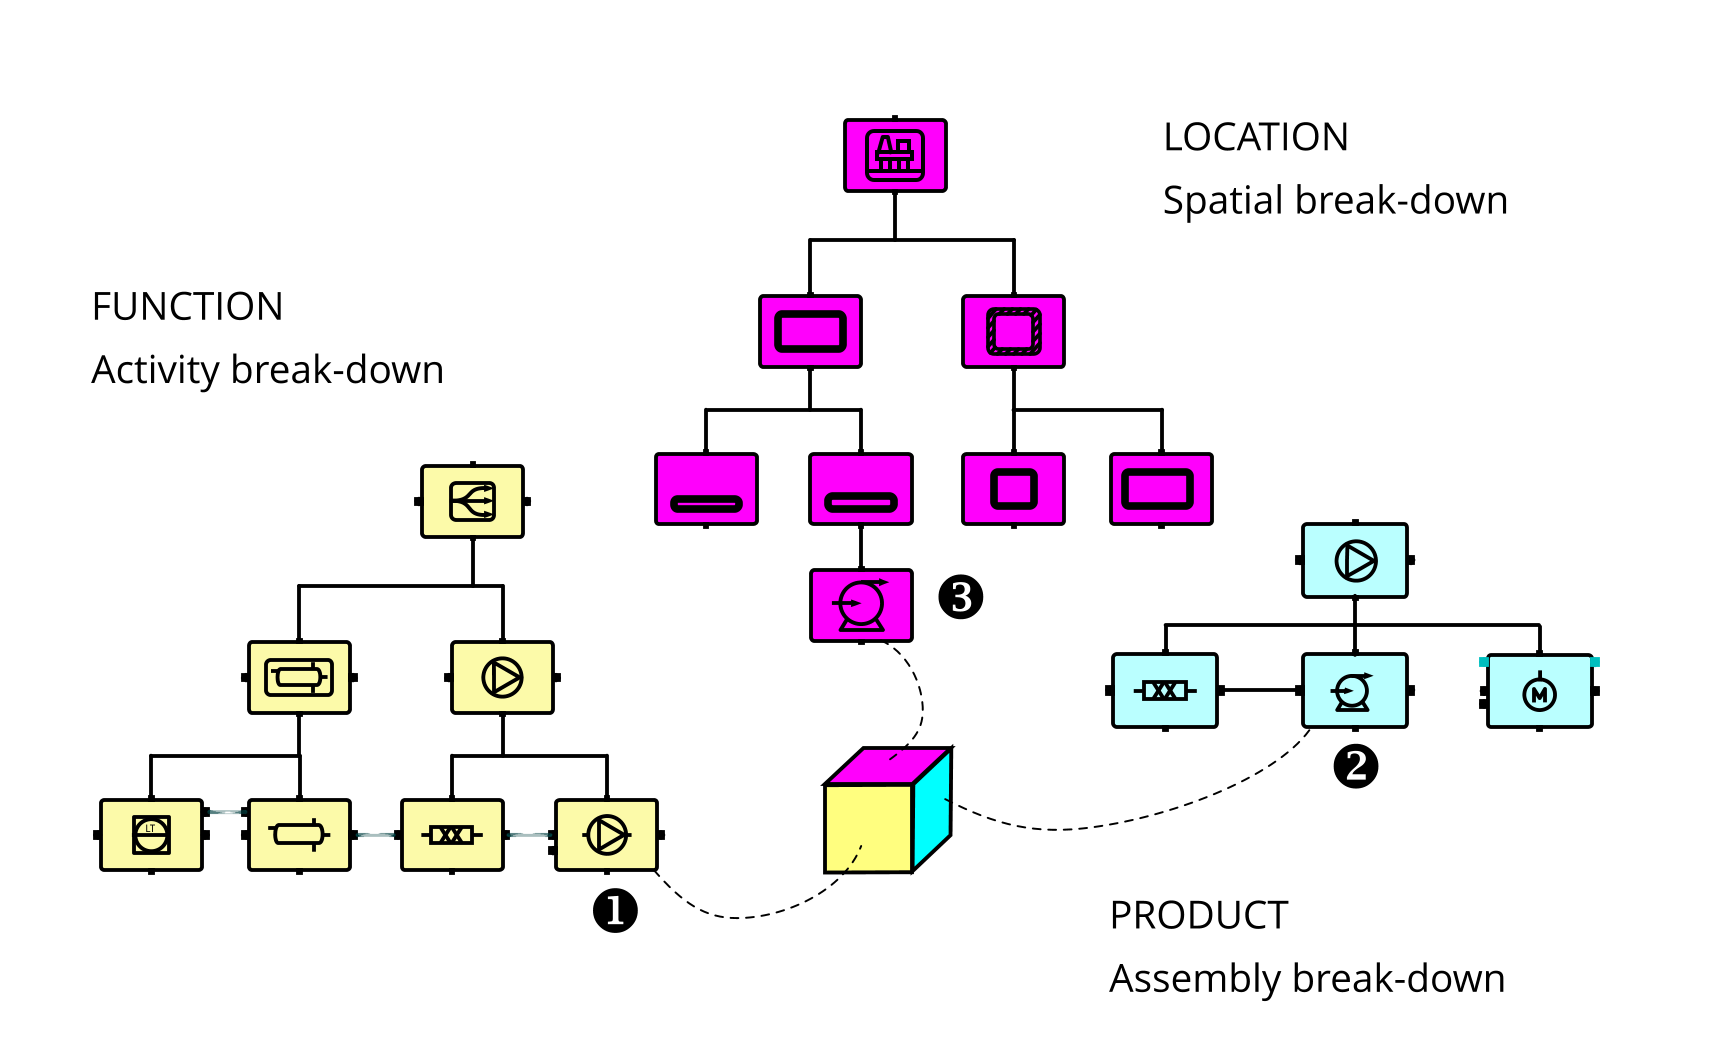
\includegraphics[width=.8\textwidth]{img/IMFmanual-img009.png}
%  \caption{Aspect Breakdowns for the Function, Location and Product aspect.}
%  \label{fig:Figure 9}
%\end{figure}


%\autoref{fig:Figure 9}; illustrates Aspect Breakdowns for the Function, Location and Product aspect. The breakdown in the Function aspect \ding{182} breaks  a main activity (separating) down into sub-activities. The Product aspect \ding{183} gives the specification of the pump as a product and the breakdown reflects how the product is \emph{part of} a larger assembly of products. The Location aspect \ding{184} is information about the space occupied by the product. The space occupied by the product is a part of a spatial breakdown, where its relative location and the requirements specific to that space is specified.

% Relations between aspects may arise when something (the cube in \autoref{fig:Figure 9} Baifan: this is confusing) has several aspects that each relate to a different aspect of the Information Model. This example revolves around the intended pumping, where \ding{182} is the
% functional aspect of the pumping, which is \emph{part of} a pumping system, which again is \emph{part of} a % separation system. 


% Observe that the concepts of system, system breakdown, and system topology are not basic concepts in IMF.
% Quite to the contrary these are complex concepts that must be modelled in a more restricted modelling language, i.e., the IMF language. In IMF the concepts of aspect, aspect breakdown, aspect topology, and inter-aspect relation
% are fundamental concepts.


\end{document}
